\documentclass[10pt]{article}
\usepackage[utf8]{inputenc}
\usepackage[T1]{fontenc}
\usepackage{amsmath}
\usepackage{amsfonts}
\usepackage{amssymb}
\usepackage[version=4]{mhchem}
\usepackage{stmaryrd}
\usepackage{graphicx}
\usepackage[export]{adjustbox}
\graphicspath{ {./images/} }

\DeclareUnicodeCharacter{21D2}{\ifmmode\Rightarrow\else{$\Rightarrow$}\fi}

\begin{document}
Contraction mapping theorem provides a very simple method for computing the value function numerically (when the closed-form solution does not)

\section*{Guess TV}
while $V \neq T V \quad$ iterate on $V$ till $V=T V \left(\begin{array}{c}V=T V \\ \text { computeTV } \\ \text { end }\end{array}\right.$

To implement it:\\
tol $=10^{-6}(\mathrm{small})$\\
$T V=$ (guess, e.g. 0 )\\
diff $=1$\\
while diff > tol

$$
\begin{aligned}
& V=T V \\
& T V=\max _{k l}\left\{F\left(k, k^{\prime}\right)+\beta V\left(k^{\prime}\right)\right\} \\
& \operatorname{dift}=\|V-T V\|
\end{aligned}
$$

sit the tolerance level to "Judge" if $V$ is suft-dose to TV

\section*{More details:}
\begin{itemize}
  \item How to define $V(k)$ (no analytucal expression)?\\
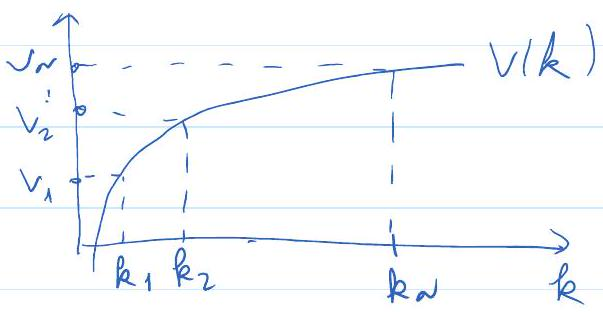
\includegraphics[max width=\textwidth, alt={}, center]{3e5e1f52-d3d3-40da-bc4a-648445fa4dde-1_312_603_1868_332}\\
create a grid:\\[0pt]
[ $k_{1} \ldots k_{N}$ ]\\
Then a function $V(k)$ is described by $\left[V_{1} \ldots V_{N}\right]$\\
(values on this grid)\\
In practice,\\
$k_{\text {grid }}=$ linspace $\left(k_{\text {mir }}, k_{\text {max }}, N\right)$ uniformly spaced Then the goal of the code is between Kmin 8 kmal to find $\left[V_{1} \ldots V_{N}\right]$ such that\\
$\left[V_{1} \ldots V_{N}\right]=\left[T V_{1} \ldots T V_{N}\right]$\\
⇒ set $k_{\text {min }}, k_{\text {max }}, N$, defince $k_{\text {grid }}$ in the beginning of the code.
  \item How to compute $|T V-V|-$ ?\\
utility values are not meaninful! ⇒\\
⇒ use "consumption equivalence"!\\
Let $C_{v}$ be cons. level:
\end{itemize}

$$
\begin{aligned}
& V=\sum_{+\infty}^{\infty} \beta^{+} u\left(c_{v}\right)=\frac{u\left(c_{v}\right)}{1-\beta} \\
& \Rightarrow \operatorname{measure}|T V-V|=\left|c_{v}-C_{T v}\right|, \text { i.e. } \\
& \max \mid \operatorname{abs}\left(u^{-1}((1-\beta) V)-u^{-1}((1-\beta) T V)\right)
\end{aligned}
$$

\begin{itemize}
  \item How to find $\max _{k^{\prime} \leq f(k)}\left\{F\left(k, k^{\prime}\right)+V\left(k^{\prime}\right)\right\}$
\end{itemize}

Most arious:

$$
\left[\begin{array}{l}
\text { for } \\
{[T} \\
\text { end }
\end{array}\right.
$$

index of the element that delivers the hignest value

Loops are slow. Can do the same in ane row using

$$
\begin{aligned}
\max & \left(\left[\begin{array}{cccc}
-F\left(k_{1}, k_{1}\right)+\beta V_{1} & F\left(k_{2}, k_{1}\right)+\beta V_{1} & \ldots & F\left(k_{N}, k_{1}\right)+\beta V_{1} \\
F\left(k_{1}, k_{2}\right)+\beta V_{2} & F\left(k_{2}, k_{2}\right)+\beta V_{2} & \ldots & F\left(k_{N}, k_{2}\right)+\beta V_{2} \\
\vdots & & & \\
F\left(k_{1}, k_{N}\right)+\beta V_{N} & F\left(k_{2}, k_{N}\right)+\beta V_{N} & \ldots & F\left(k_{N}, k_{N}\right)+\beta V_{N}
\end{array}\right]\right) \\
& (N \times N) \text { matric }
\end{aligned}
$$

would find the max in every colemn to buld such a matrix:\\
$k k=k r o n(k$ grid, ones $(N, 1))$\\[0pt]
[TV ind g] $=\max \left(F\left(k k, k k^{\prime}\right)+\beta \operatorname{kror}\left(V^{\prime}\right.\right.$, ones $\left.(1, N)\right)$\\
this line replaces the whole loop \& computes TV for a given V

Finally, notice that $F\left(k k, k k^{\prime}\right)$ depends on the gridenly ⇒ no need to recompute it inside the while loop for any new greess of $V$.

⇒ stuncture the coder as follows:\\
set tolerance tol\\
define Kegrid\\
find $k k$, $u$ til $=F\left(k k, k k^{\prime}\right)$\\
guss TV\\
set diff $=1$ (any $>$ tol)\\
while diff > tol

$$
\begin{aligned}
& V=T V \\
& {[T V \text { ind } g]=\max \ldots} \\
& \text { dift }=\max \left(\operatorname{abs}\left(u^{-1}((1-\beta) V)-u^{-1}((1-\beta) T V)\right)\right)
\end{aligned}
$$

end.\\
Remark: $\quad k$ grid (ind $g$ ) is the policy function!\\
(e.g. plot (kgrid, kgrig(indg)) would phot $k^{\prime}=g(k)$

Some things to worry about:\\
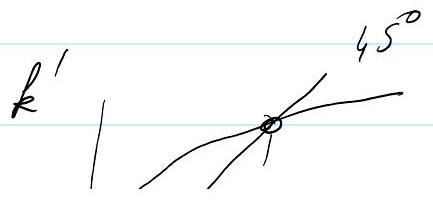
\includegraphics[max width=\textwidth, alt={}, center]{3e5e1f52-d3d3-40da-bc4a-648445fa4dde-3_204_433_2437_1625}

\section*{Some things to worry about:}
(1) $k_{\max }\left(k_{N}\right)$ must be large enough $\left(k_{\text {max }}>k^{*}\right)$\\
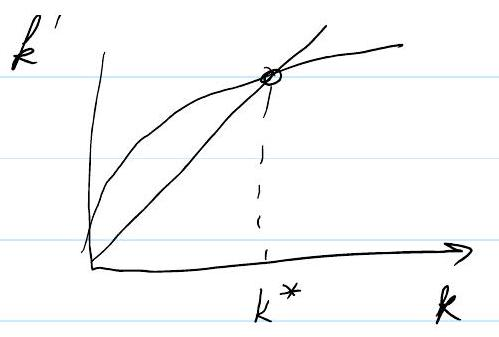
\includegraphics[max width=\textwidth, alt={}, center]{3e5e1f52-d3d3-40da-bc4a-648445fa4dde-4_337_499_110_1625}\\
check that $k_{\text {max }}$ is not binding $\left(g(k)<k_{\text {max }}, \forall k\right)$\\
(2) N-large enough\\
increase $N \Rightarrow V, g$ must not be significanly affecter 1\\
(3) tol must be small enough\\
deceease tol, make sure that $V, g$ are not much affected

Sometimes the brute-force value function iteration is too slow (multiple state variables "curse of dimensionality")\\
$\Rightarrow \exists$ tricks to speed up the algorytm:

\begin{enumerate}
  \item Evaluate $V$ on a sparser grid of $\left[k_{1} \ldots k_{m}\right]$.
\end{enumerate}

Interpolate $V$ on the intermediate levels of $k$ (use interp1 in Matlab)\\
choose optimal $k^{\prime}$ from a denser grid.\\
The grid for $k$ may be chosen unevenly: more grid points in the region in which $V$ is more concave (small $k$ )\\
2) Use the properties of $V(k), g(k)$ in your computas. lif you can establish analytical properties)\\
Example: $g(k)$-monotone $\Rightarrow$\\
the set of $k^{\prime}$ over which you need to search adjusts with $k$\\
(fewer computations will be made ⇒ ) faster\\
3) Howard's Improvement algorythm:\\
(a) compute $g / k$ ) for a given $V$-guess\\
(b) compute $V(k)$ induced by $g(k)$

$$
V(k)=F(k, g(k))+\beta V(g / k)) \quad \text { (nomax). }
$$

Ov apply the RHS of the above max is true consuming)\\
10-20 times, not till converge to the solution

\begin{itemize}
  \item repeat $(a) t(b)$ till $g(k)$ das not change.
\end{itemize}

\section*{(sometimes does not converge)}
\begin{enumerate}
  \setcounter{enumi}{3}
  \item Solve numerically the Euler Equation
  \item Continuous time formulation -- easier to solve (see work of Ben Moll)
  \item neural networks methods to approximate value function or policy functions (using eg Deep Learning Toolbox in Matlab)
\end{enumerate}

\end{document}